\documentclass{beamer}\usepackage[]{graphicx}\usepackage[]{color}
%% maxwidth is the original width if it is less than linewidth
%% otherwise use linewidth (to make sure the graphics do not exceed the margin)
\makeatletter
\def\maxwidth{ %
  \ifdim\Gin@nat@width>\linewidth
    \linewidth
  \else
    \Gin@nat@width
  \fi
}
\makeatother

\definecolor{fgcolor}{rgb}{0.345, 0.345, 0.345}
\newcommand{\hlnum}[1]{\textcolor[rgb]{0.686,0.059,0.569}{#1}}%
\newcommand{\hlstr}[1]{\textcolor[rgb]{0.192,0.494,0.8}{#1}}%
\newcommand{\hlcom}[1]{\textcolor[rgb]{0.678,0.584,0.686}{\textit{#1}}}%
\newcommand{\hlopt}[1]{\textcolor[rgb]{0,0,0}{#1}}%
\newcommand{\hlstd}[1]{\textcolor[rgb]{0.345,0.345,0.345}{#1}}%
\newcommand{\hlkwa}[1]{\textcolor[rgb]{0.161,0.373,0.58}{\textbf{#1}}}%
\newcommand{\hlkwb}[1]{\textcolor[rgb]{0.69,0.353,0.396}{#1}}%
\newcommand{\hlkwc}[1]{\textcolor[rgb]{0.333,0.667,0.333}{#1}}%
\newcommand{\hlkwd}[1]{\textcolor[rgb]{0.737,0.353,0.396}{\textbf{#1}}}%
\let\hlipl\hlkwb

\usepackage{framed}
\makeatletter
\newenvironment{kframe}{%
 \def\at@end@of@kframe{}%
 \ifinner\ifhmode%
  \def\at@end@of@kframe{\end{minipage}}%
  \begin{minipage}{\columnwidth}%
 \fi\fi%
 \def\FrameCommand##1{\hskip\@totalleftmargin \hskip-\fboxsep
 \colorbox{shadecolor}{##1}\hskip-\fboxsep
     % There is no \\@totalrightmargin, so:
     \hskip-\linewidth \hskip-\@totalleftmargin \hskip\columnwidth}%
 \MakeFramed {\advance\hsize-\width
   \@totalleftmargin\z@ \linewidth\hsize
   \@setminipage}}%
 {\par\unskip\endMakeFramed%
 \at@end@of@kframe}
\makeatother

\definecolor{shadecolor}{rgb}{.97, .97, .97}
\definecolor{messagecolor}{rgb}{0, 0, 0}
\definecolor{warningcolor}{rgb}{1, 0, 1}
\definecolor{errorcolor}{rgb}{1, 0, 0}
\newenvironment{knitrout}{}{} % an empty environment to be redefined in TeX

\usepackage{alltt}
\IfFileExists{upquote.sty}{\usepackage{upquote}}{}
\begin{document}

\title{Chance the Rapper - Coloring Book Wordcloud}
\author{Bill Fisher}

\begin{frame}
  \titlepage
\end{frame}

\begin{frame}
  \frametitle{Outline}
    \tableofcontents
\end{frame}

\section{Install and Load Libraries}
\begin{frame}[fragile]
  \frametitle{Install and Load Libraries}
    \begin{itemize}
      \item<1->
\begin{knitrout}
\definecolor{shadecolor}{rgb}{0.969, 0.969, 0.969}\color{fgcolor}\begin{kframe}
\begin{alltt}
\hlkwd{library}\hlstd{(dplyr)}
\end{alltt}
\end{kframe}
\end{knitrout}
      \item<2->
\begin{knitrout}
\definecolor{shadecolor}{rgb}{0.969, 0.969, 0.969}\color{fgcolor}\begin{kframe}
\begin{alltt}
\hlkwd{library}\hlstd{(tidytext)}
\end{alltt}
\end{kframe}
\end{knitrout}
      \item<3->
\begin{knitrout}
\definecolor{shadecolor}{rgb}{0.969, 0.969, 0.969}\color{fgcolor}\begin{kframe}
\begin{alltt}
\hlkwd{library}\hlstd{(wordcloud)}
\end{alltt}
\end{kframe}
\end{knitrout}
      \item<4->
\begin{knitrout}
\definecolor{shadecolor}{rgb}{0.969, 0.969, 0.969}\color{fgcolor}\begin{kframe}
\begin{alltt}
\hlkwd{library}\hlstd{(tm)}
\end{alltt}
\end{kframe}
\end{knitrout}
      \item<5->
\begin{knitrout}
\definecolor{shadecolor}{rgb}{0.969, 0.969, 0.969}\color{fgcolor}\begin{kframe}
\begin{alltt}
\hlkwd{library}\hlstd{(stringr)}
\end{alltt}
\end{kframe}
\end{knitrout}
    
    \end{itemize}
\end{frame}

\section{Scan in Text Document}
\begin{frame}[fragile]
  \frametitle{Scan in Text Document}
\begin{knitrout}
\definecolor{shadecolor}{rgb}{0.969, 0.969, 0.969}\color{fgcolor}\begin{kframe}
\begin{alltt}
\hlstd{chance_cb}\hlkwb{<-}\hlkwd{scan}\hlstd{(}\hlstr{'chance_coloringbook.txt'}\hlstd{,}\hlkwc{what}\hlstd{=}\hlkwd{character}\hlstd{(),}\hlkwc{sep}\hlstd{=}\hlstr{'\textbackslash{}n'}\hlstd{)}
\hlkwd{head}\hlstd{(chance_cb)}
\end{alltt}
\begin{verbatim}
## [1] "All We Got "                                               
## [2] "And we back"                                               
## [3] "And we back, and we back, and we back, and we back, and we"
## [4] "And we back, and we back, na, na, na"                      
## [5] "This ain't no intro, this the entree"                      
## [6] "Hit that intro with Kanye and sound like Andr�"
\end{verbatim}
\end{kframe}
\end{knitrout}
\end{frame}

\section{Unpack the Words}
\begin{frame}[fragile]
  \frametitle{Unpack the Words}
\begin{knitrout}
\definecolor{shadecolor}{rgb}{0.969, 0.969, 0.969}\color{fgcolor}\begin{kframe}
\begin{alltt}
\hlstd{chance_cb}\hlkwb{<-}\hlkwd{data_frame}\hlstd{(}\hlkwc{line}\hlstd{=}\hlnum{1}\hlopt{:}\hlnum{1038}\hlstd{,} \hlkwc{text}\hlstd{=chance_cb)}
\hlstd{chance_words}\hlkwb{<-}\hlstd{chance_cb}\hlopt
  \hlkwd{unnest_tokens}\hlstd{(word, text)}
\end{alltt}
\end{kframe}
\end{knitrout}
\end{frame}

\section{Remove Stop Words}
\begin{frame}[fragile]
  \frametitle{Remove Stop Words}
\begin{knitrout}
\definecolor{shadecolor}{rgb}{0.969, 0.969, 0.969}\color{fgcolor}\begin{kframe}
\begin{alltt}
\hlstd{chance_words}\hlkwb{<-}\hlstd{chance_words}\hlopt
  \hlkwd{filter}\hlstd{(}\hlopt{!}\hlstd{(word} \hlopt \hlstd{stop_words}\hlopt{$}\hlstd{word))}
\hlkwd{print}\hlstd{(chance_words,}\hlkwc{n}\hlstd{=}\hlnum{5}\hlstd{)}
\end{alltt}
\begin{verbatim}
## # A tibble: 2,478 x 2
##    line   word
##   <int>  <chr>
## 1     4     na
## 2     4     na
## 3     4     na
## 4     5  intro
## 5     5 entree
## # ... with 2,473 more rows
\end{verbatim}
\end{kframe}
\end{knitrout}
\end{frame}

\section{Obtain Word Frequency}
\begin{frame}[fragile]
  \frametitle{Obtain Word Frequency}
\begin{knitrout}
\definecolor{shadecolor}{rgb}{0.969, 0.969, 0.969}\color{fgcolor}\begin{kframe}
\begin{alltt}
  \hlstd{chance_word_freq}\hlkwb{<-}\hlstd{chance_words}\hlopt
    \hlkwd{group_by}\hlstd{(word)}\hlopt
    \hlkwd{summarize}\hlstd{(}\hlkwc{count}\hlstd{=}\hlkwd{n}\hlstd{())}
  \hlkwd{print}\hlstd{(chance_word_freq,}\hlkwc{n}\hlstd{=}\hlnum{2}\hlstd{)}
\end{alltt}
\begin{verbatim}
## # A tibble: 1,127 x 2
##    word count
##   <chr> <int>
## 1     0     2
## 2     1     2
## # ... with 1,125 more rows
\end{verbatim}
\end{kframe}
\end{knitrout}
\end{frame}

\section{Generate Wordcloud}
\begin{frame}[fragile]
  \frametitle{Generate Wordcloud}
\begin{knitrout}
\definecolor{shadecolor}{rgb}{0.969, 0.969, 0.969}\color{fgcolor}\begin{kframe}
\begin{alltt}
  \hlcom{#wordcloud(chance_word_freq$word, }
  \hlcom{#chance_word_freq$count, min.freq=5)}

  \hlcom{#Note: Displaying compiled Wordcloud in next slide so }
  \hlcom{#figure displays properly on screen}
\end{alltt}
\end{kframe}
\end{knitrout}
\end{frame}

\section{Generate Wordcloud}
\begin{frame}[fragile]
  \frametitle{Generate Wordcloud}
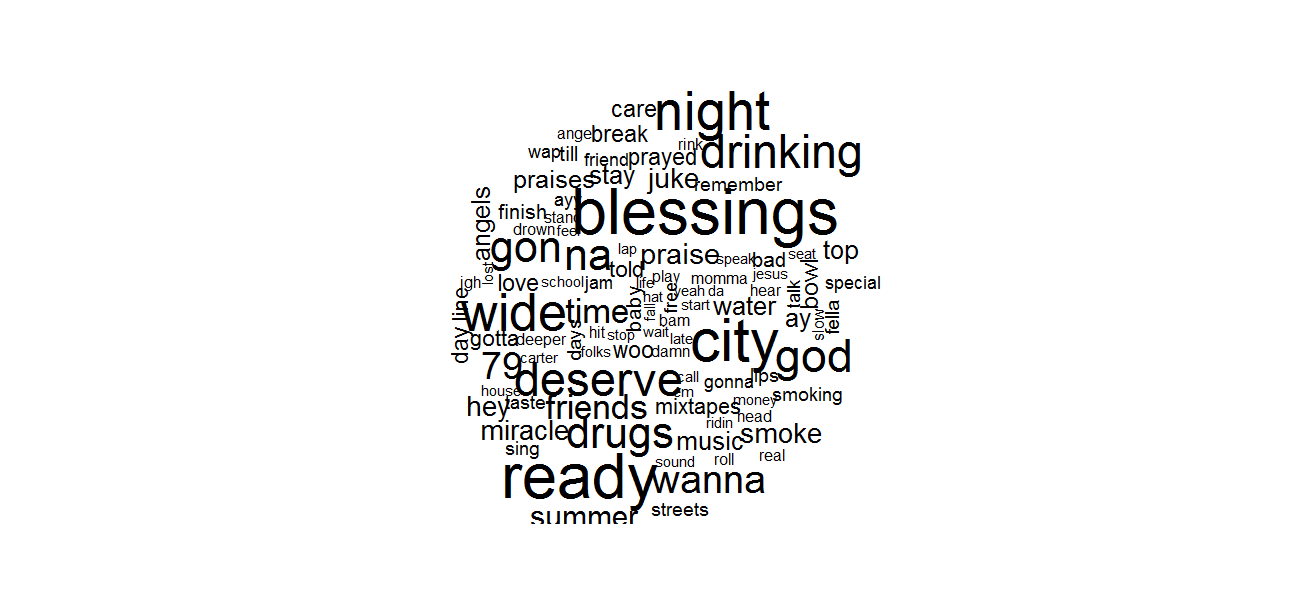
\includegraphics[scale=0.25]{Chance_Rplot}
\end{frame}
  
\end{document}
